\section{Sterowanie jednostkami (Zofia Sosińska)}\label{chap:mb}
Niektóre informacje są najlepiej spełniają swoja rolę, gdy pojawiają się tylko na chwilę. Zdarza się, że gracz potrzebuje przypomnienia
o nich przez krótką chwilę podejmowania decyzji, a po niej nie ma potrzeby, aby grafika zajmowała cenne miejsce na ekranie, zasłaniając świat gry.
Takie dane opisują sytuacje, gdy gracz wydaje komendę podwładnym jednostkom. Dzieje się to prawdopodobnie podczas bitwy, więc użytkownik musi skupić się
na taktyce walki i nie chce być rozpraszany. Rozsądnym rozwiązaniem w tej sytuacji jest podpowiedzenie mu, gdy wydaje sam rozkaz, ale nieprzeszkadzanie zasłanianiem ekranu,
gdy skupia się na innym aspekcie sytuacji.

Gra Mount\&Blade tureckiego studia TaleWorlds Entertainment, wydana przez Paradox Interactive rozwiązuje problem sterowania jednostkami w zbalansowany sposób.
Poprzez cyfry 0-4 wybiera grupę, do której się odnosi np. łuczników. Po naciśnięciu jednego z przycisków, z boku ekranu pojawia się lista dostępnych komend. Przez 
klawisze F1-F11 wydaje konkretny rozkaz np. odwrót. Sztuczna inteligencja postaci zajmuje się już samym wykonaniem czynności. Gracz nie martwi się,
czy jednostki znajdą optymalną drogę, będą celować w przeciwników, czy z nimi walczyć.


\begin{figure}[h!tbp]
    \centering
    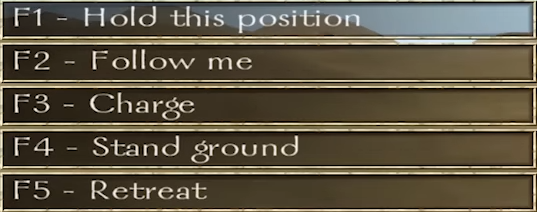
\includegraphics[width=0.9\textwidth]{images/ui/commandsMountBla.png}
    \caption{Wykaz dostępnych rozkazów z gry Mount\&Blade.}\label{fig:MountnBlade}
    \label{fig:mnb}
\end{figure}
